\section{Wprowadzenie}
\label{sec:Wprowadzenie}
\begin{flushleft}

    Jesteśmy studentami, którzy chcieli pomóc innym studentom w trudnym czasie tj. sesja. \\ 
    Nasz projekt to aplikacja o nazwie StudUnity. Jest ona całkowicie darmowa. Zawiera wszystkie najważniejsze notatki z wykładów oraz laboratoriów. \\ Naszą główną inspiracją była aplikacja wspirająca uczniów szkół podstawowych.
    
\begin{figure}[htbp]
    \centering
    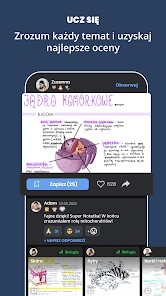
\includegraphics[width=0.3\textwidth]{pictures/inspriracje.jpg}
    \caption{inspiracje}
    \label{fig:inspiracje}
\end{figure}

\noindent Obrazek powyższy ukazuje inspiracje do powstania naszej aplikacji.\\
(see inspiracje~\ref{fig:inspiracje}).
\newpage
\vspace {0.60cm}

    Chyba każdy z nas spotkał kiedyś takiego smutnego studenta na swojej drodze. Często przechodzimy obok i nawet nie zapytamy czemu jest studentem lub czemu łzy mu napływają do oczu. 
    Gdybyśmy się tylko dopytali okazało by się w 90 procentach, że gościu lub gościówa nie zdali kolasa. 
    
\vspace {0.60cm}

    {{\large TERAZ JUŻ WIESZ CO TAKIM STUDENTOM DORADZIĆ   }}
    {{\Large POLEĆ IM STUDUNITY I ZAPROŚ NA PIWO}}
    
\vspace {0.50cm}

    (bo to jednak biedny student, więc nie tyle nie zdał, co i nie ma pieniędzy, żeby się pocieszyć)
    
\vspace {0.55cm}

Dzięki Tobie student już nigdy nie będzie płakał z powodu nauki i uczelni.

\vspace {0.50cm}
{{\Large WYSTARCZY TYLKO JEDNO SŁOWO,\\ 
        A STUDENT MOŻE WYGLĄDAĆ TAK:}}

\begin{figure}[htbp] 
    \centering
    
\includegraphics[width=0.5\textwidth]{pictures/zadowolony-student.JPG} 
    \caption{Takiej radości w życiu nie spotkasz}
    \label{fig:radosc}
\end{figure}

\end{flushleft}